% !TEX root = ../thesis.tex

\chapter{Fusing of the two measurement sources}

Lorem ipsum dolor sit amet, consectetuer adipiscing elit, sed diam nonummy nibh euismod tincidunt ut laoreet dolore magna aliquam erat volutpat. Ut wisi enim ad minim veniam, quis nostrud exerci tation ullamcorper suscipit lobortis nisl ut aliquip ex ea commodo consequat. Duis autem vel eum iriure dolor in hendrerit in vulputate velit esse molestie consequat, vel illum dolore eu feugiat nulla facilisis at vero et accumsan et iusto odio dignissim qui blandit.

\section{Extended Kalman Filter (EKF)}

\subsection{System Model}

The state $\vec x = [\vec r, \vec v]^T$ of our model consists of a position $\vec r \in \mathbb{R}^3$ and a velocity $\vec v \in \mathbb{R}^3$.
The discrete process model with timestep $\Delta T$ is given by
\begin{equation}
	\vec x(k) = \textbf{A} \vec x(k-1) + \vec v(k-1)
\end{equation}
where 
\begin{align}
	\textbf{A} =
	\begin{pmatrix}
		\textbf{I}_3 & \Delta \textbf{T}\\
		\textbf{0} & \textbf{I}_3
	\end{pmatrix}
\end{align} 

and
\begin{equation}
	\vec v(k-1) \sim \mathcal{N}(\vec 0, \textbf{Q}(k-1))
\end{equation}
where
\begin{align}
	\textbf{Q}(k-1) =
	\begin{pmatrix}
		\textbf{0} & \textbf{0}\\
		\textbf{0} & \textbf{q}_v(k-1)
	\end{pmatrix}
\end{align}
and $\textbf{q}_v \in \mathbb{R}^{3\times3}$ is the velocity covariance of the process noise.
There are two possible measurements. The first measurement is a direct measurement of the state $\vec x$ from ultra-wideband (UWB) trilateration:
\begin{equation}
	\vec z_1(k) = \textbf{H}_1 \vec x(k) + \vec \omega_1(k)\\
\end{equation}
where
$$\textbf{H}_1 = \textbf{I}_6$$
and
$$\vec \omega_1(k) \sim \mathcal{N}(\vec 0, \textbf{R}_1)$$
where $\textbf{R}_1 \in \mathbb{R}^{6\times6}$ is the covariance of the UWB measurement.
The second measurement is a projection of the position $\vec r$ as seen by a camera:
\begin{align}
	\vec z_2(k) = \textbf{H}_2(\vec x(k)) + \vec \omega_2(k)\\
	\textbf{H}_2(\vec x) = [\frac{x_1}{x_3}, \frac{x_2}{x_3}]^T \in \mathbb{R}^2\\
	\vec \omega_2(k) \sim \mathcal{N}(\vec 0, \textbf{R}_2)
\end{align}
where $\textbf{R}_2 \in \mathbb{R}^{2\times2}$ is the covariance of the camera measurement.

\subsection{The Extended Kalman Filter steps}
There are two steps which have to be performed in an iterative fashion when running the Extended Kalman Filter.

\subsubsection{Step 1: Prior update/Prediction step}
In the first step, a prediction for the mean of the states $\hat{\vec x}_p(k)$ and the co-variance matrix $\textbf{P}_p(k)$ is calculated from the linearized system model.
\begin{align}
	\hat{\vec x}_p(k) &= \textbf{A}\vec x(k-1)\\
	\textbf{P}_p(k) &= \textbf{A}(k-1) \textbf{P}_m(k-1) \textbf{A}^T(k-1) + \textbf{L}(k-1) \textbf{Q}(k-1) \textbf{L}^T(k-1) \label{eq:ekf_s1}
\end{align}
where
\begin{align}
	\textbf{A}(k-1) & =  \frac{\partial}{\partial \vec x} \big(\textbf{A} \vec x(k-1) + \vec v(k-1)\big)\\
	& = \textbf{I}_6\\
	\textbf{L}(k-1) & = \frac{\partial}{\partial \vec v} \big( \textbf{A} \vec x(k-1) + \vec v(k-1)\big)\\
	& = \textbf{I}_6
\end{align}
and with the initial values $\hat{\vec x}_m(0) = x_0$ and $\textbf{P}_m(0) = \textbf{0}$.
Therefore equation \ref{eq:ekf_s1} becomes
$$\textbf{P}_p(k) = \textbf{P}_m(k-1) + \textbf{Q}(k-1) = \textbf{P}_m(k-1) + \textbf{Q}$$

\subsubsection{Step 2: A posteriori update/Measurement update step}
In the second step, the information gained from the measurements are used to perform an a posteriori update, resulting in a updated mean of the states $\hat{\vec x}_m(k)$and an updated co-variance matrix $\textbf{P}_m(k)$.
\begin{align}
	\textbf{K}(k) = \textbf{P}_p(k) \textbf{H}^T(k) \Big( \textbf{H}(k) \textbf{P}_p(k) \textbf{H}^T(k) + \textbf{M}(k) \textbf{R}(k) \textbf{M}^T(k)\Big)^{-1} \label{eq:ekf_s2}\\
	\hat{\vec x}_m(k) = \hat{\vec x}_p(k) + \textbf{K}(k) \Big( \vec z(k) - \begin{bmatrix}
	\textbf{H}_1 \hat{\vec x}(k)\\
	\textbf{H}_2(\hat{\vec x}(k))
	\end{bmatrix} \Big)\\
	\textbf{P}_m(k) = \big( \textbf{I} - \textbf{K}(k)\textbf{H}(k)\big) \textbf{P}_p(k)
\end{align}
where
\begin{align}
	\textbf{H}(k) &= \begin{bmatrix}
		\frac{\partial}{\partial \vec x} \big( \textbf{H}_1 \hat{\vec x}(k) + \vec \omega_1(k) \big)\\
		\frac{\partial}{\partial \vec x} \big( \textbf{H}_2(\hat{\vec x}(k)) + \vec \omega_2(k) \big)
	\end{bmatrix}\\
	&= \begin{bmatrix}
		\textbf{I}_6\\
		\frac{1}{\hat{x}_3} & 0 & -\frac{\hat{x}_1}{\hat{x}^2_3} & 0 & 0 & 0\\
		0 & \frac{1}{\hat{x}_3} & -\frac{\hat{x}_2}{\hat{x}^2_3} & 0 & 0 & 0
	\end{bmatrix}\\
	\textbf{M}(k) &= \begin{bmatrix}
		\frac{\partial}{\partial \vec \omega} \big( \textbf{H}_1 \hat{\vec x}(k) + \vec \omega_1(k) \big)\\
		\frac{\partial}{\partial \vec \omega} \big( \textbf{H}_2(\hat{\vec x}(k)) + \vec \omega_2(k) \big)
	\end{bmatrix}\\
	&= \textbf{I}_8
\end{align}
Therefore equation \ref{eq:ekf_s2} becomes
$$\textbf{K}(k) = \textbf{Q} \textbf{H}^T(k) \Big( \textbf{H}(k) \textbf{Q} \textbf{H}^T(k) + \begin{bmatrix}
	\textbf{R}_1 & \textbf{0}\\
	\textbf{0} &\textbf{R}_2
\end{bmatrix} \Big)^{-1}$$

\subsection{Another Subsection}

\begin{table}
    \centering
    \begin{tabular}{|l|p{0.4\linewidth}|}
    \hline
    \emph{Quant.} & \emph{Ingredient}\\
    \hline
		200g &Wei{\ss}mehl\\
		1/4  &Packung Frischhefe\\
		4EL  &lauwarme Milch\\
		4EL  &�l\\
		1TL  &Zucker\\
		1TL  &Salz\\
		&lauwarmes Wasser\\
    \hline
    \end{tabular}
    \caption[Flammkuchenteig]{Flammkuchenteig. The ingredients have to be carefully chosen.\label{tab:mytable}}
\end{table}
%
Lorem ipsum dolor sit amet, consectetuer adipiscing elit, sed diam nonummy nibh euismod tincidunt ut laoreet dolore magna aliquam erat volutpat. Ut wisi enim ad minim veniam, quis nostrud exerci tation ullamcorper suscipit lobortis nisl ut aliquip ex ea commodo consequat, see Table~\ref{tab:mytable}. Duis autem vel eum iriure dolor in hendrerit in vulputate velit esse molestie consequat, vel illum dolore eu feugiat nulla facilisis at vero et accumsan et iusto odio dignissim qui blandit praesent luptatum zzril delenit augue duis dolore te feugait nulla facilisi. Lorem ipsum dolor sit amet, consectetuer adipiscing elit, sed diam,
see Figure~\ref{fig:voldiff}~(a).
%
\begin{figure}
    \centering
    \setlength{\tabcolsep}{0.0130\linewidth}
    \begin{tabular}{@{}cc@{}}
    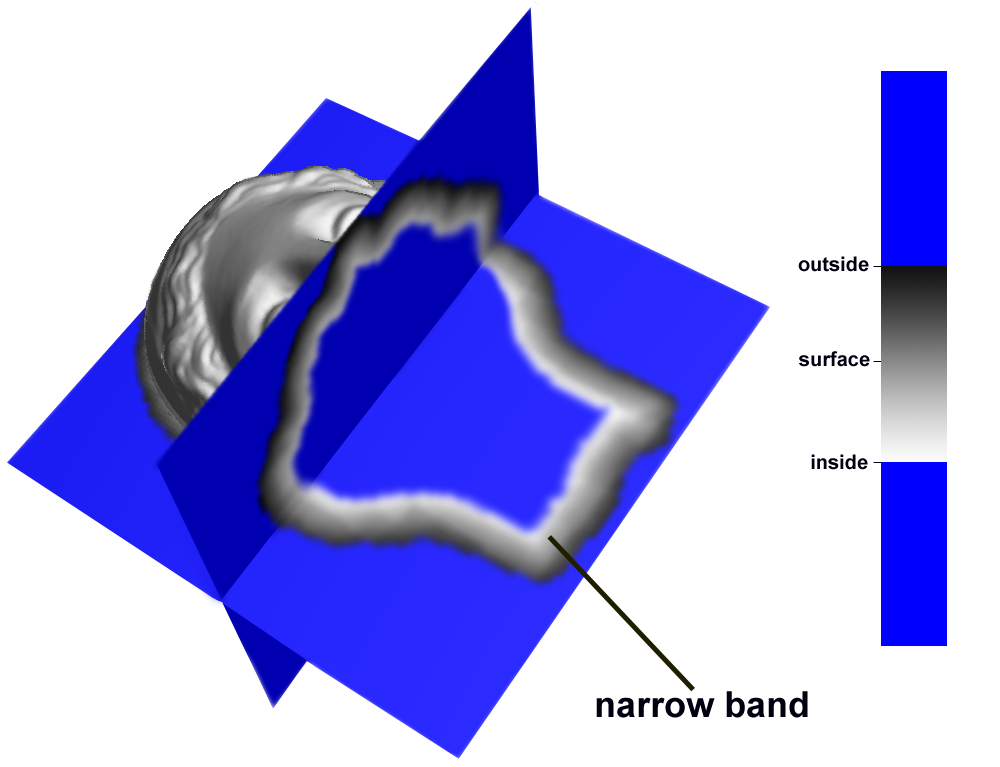
\includegraphics[width=0.487\linewidth]{figures/IgeaNarrowBand}&
    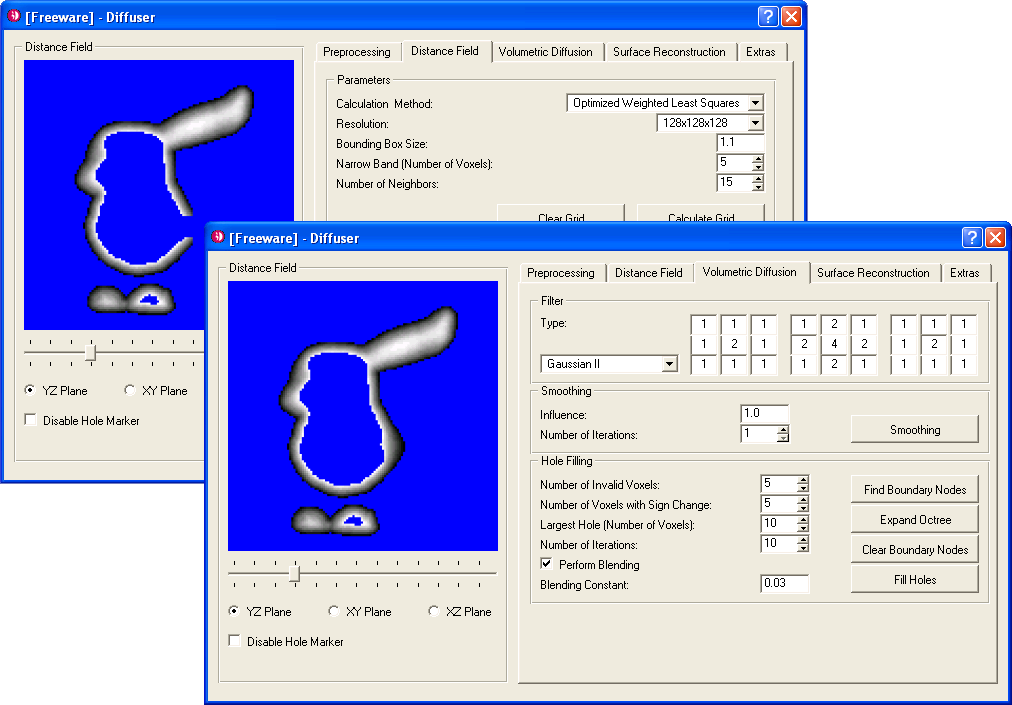
\includegraphics[width=0.487\linewidth]{figures/voldiff_ui}\\
    (a)&(b)\\
    \end{tabular}
    \caption[Volumetric diffusion]{Volumetric diffusion.
    	  \textup{(a)} Slices of the distance volume reveal the narrow band.
			  \textup{(b)} The user interface of the automatic hole filling
        tool allows to fine-tune the algorithm.
        The volumetric representation can be previewed before
        surface reconstruction.%
      \label{fig:voldiff}}
\end{figure}
%
Isn't it?

\begin{figure}[!htb]
	\centering
	\subfigure[Caption first.]{\label{fig:test1}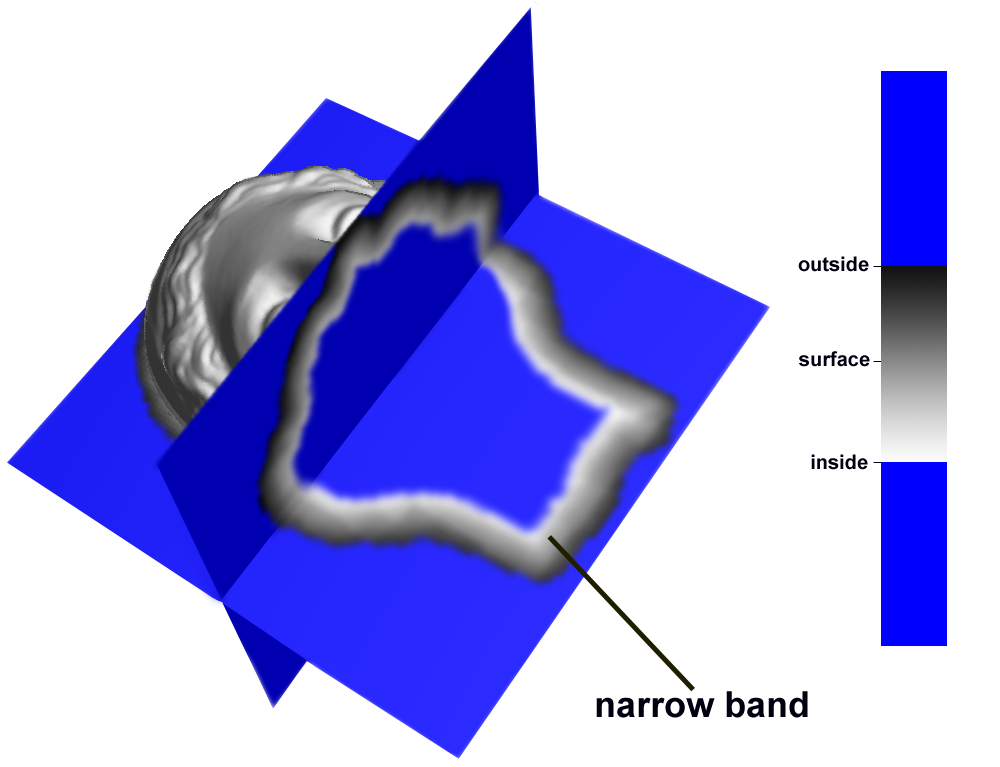
\includegraphics[width=0.3\textwidth]{figures/IgeaNarrowBand}} \hfill
	\subfigure[Caption second.]{\label{fig:test2}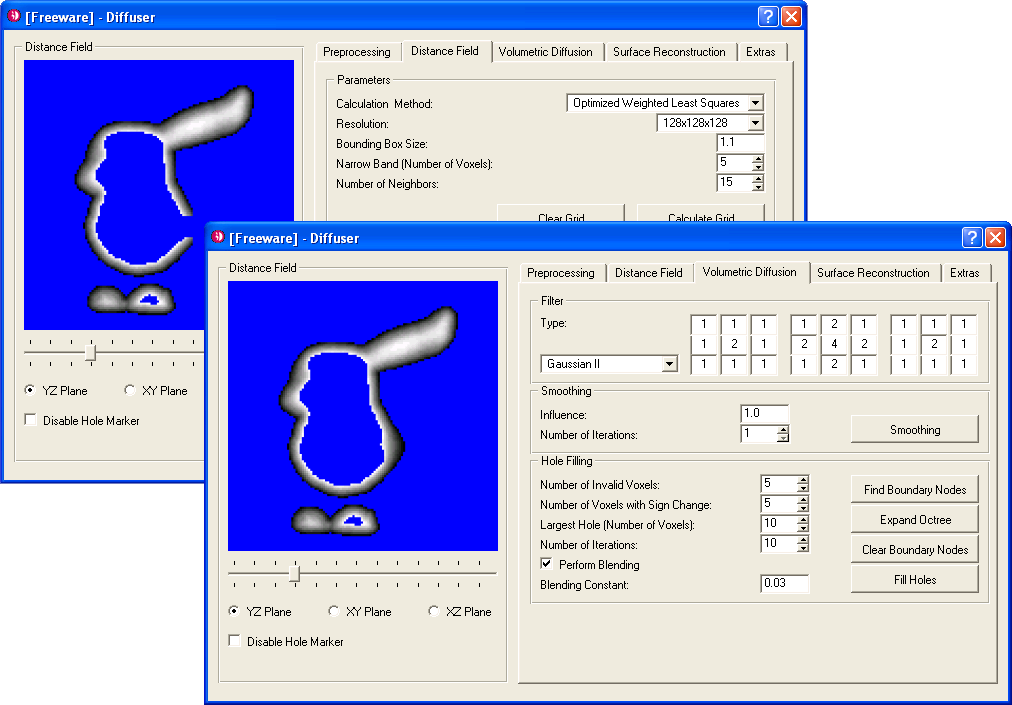
\includegraphics[width=0.3\textwidth]{figures/voldiff_ui}}
	\caption[Caption both]{Caption of both \subref{fig:test1}, \subref{fig:test2}.}
	\label{fig:bothfigures}
\end{figure}


Lorem ipsum dolor sit amet, consectetuer adipiscing elit, sed diam nonummy nibh euismod tincidunt ut laoreet dolore magna aliquam erat volutpat. Ut wisi enim ad minim veniam, quis nostrud exerci tation ullamcorper suscipit lobortis nisl ut aliquip ex ea commodo consequat. Duis autem vel eum iriure dolor in hendrerit in vulputate velit esse molestie consequat, vel illum dolore eu feugiat nulla facilisis at vero et accumsan et iusto odio dignissim qui blandit praesent luptatum zzril delenit augue duis dolore te feugait nulla facilisi. Lorem ipsum dolor sit amet, consectetuer adipiscing elit, sed diam 

\section{Second Section}

Lorem ipsum dolor sit amet, consectetuer adipiscing elit, sed diam nonummy nibh euismod tincidunt ut laoreet dolore magna aliquam erat volutpat. Ut wisi enim ad minim veniam, quis nostrud exerci tation ullamcorper suscipit lobortis nisl ut aliquip ex ea commodo consequat. Duis autem vel eum iriure dolor in hendrerit in vulputate velit esse molestie consequat, vel illum dolore eu feugiat nulla facilisis at vero et accumsan et iusto odio dignissim qui blandit praesent luptatum zzril delenit augue duis dolore te feugait nulla facilisi. Lorem ipsum dolor sit amet, consectetuer adipiscing elit, sed diam nonummy nibh euismod tincidunt ut laoreet dolore magna aliquam erat volutpat. Ut wisi enim ad minim veniam, quis nostrud exerci tation ullamcorper suscipit lobortis nisl ut aliquip ex ea commodo consequat. Duis autem vel eum iriure dolor in hendrerit in vulputate velit esse molestie consequat, vel illum dolore eu feugiat nulla facilisis at vero et accumsan et iusto odio dignissim qui blandit
